\setlength{\tabcolsep}{10pt}

\begin{frame}{Attivit\`a svolta}
\begin{enumerate}

    \item Studio di soluzioni per web scraping da fonti social network (Facebook ed Instagram)
    \item Identificazione del contrasto attuato dalle piattaforme
    \item Sviluppo connettori di scraping
    \item Sviluppo metodologie di elusione dei controlli
\end{enumerate}
    
\end{frame}



\begin{frame}{Web Scraping}
Attività di \alert{raccolta automatica} di dati da Internet attraverso:
\begin{itemize}
    \item Application Programming Interface
    \item Richieste HTTP GET
    \item Tecniche dedicate
\end{itemize}\leavevmode\newline

\begin{figure}
  \begin{center}
  \includesvg[width=260pt]{images/scraper.svg}
\end{center}
\end{figure}
\end{frame}


\begin{frame}{Aspetti legali e uso dei dati}
L'attivit\`a rientra in una \alert{``zona grigia''} della legalit\`a in quanto non espressamente definita da alcuna norma.
\begin{itemize}
    \item General Data Protection Regulation (GDPR - Europa)
    \item Computer Fraud and Abuse Act (CFAA - USA)
    \item Termini di servizio
\end{itemize}\leavevmode\newline
I possibili \alert{casi d'uso} dei dati estratti rientrano in settori investigativi e di Open Source Intelligence
\end{frame}




\begin{frame}{Connettori sviluppati}
\begin{columns}
\begin{column}{0.5\textwidth}
\centering
\alert{Facebook}\\
\begin{itemize}
    \item Tool open source ``facebook-scraper''
    \item No API ufficiali
\end{itemize}
\end{column}

\begin{column}{0.5\textwidth}
\centering
\alert{Instagram}\\
\begin{itemize}
    \item Tool open source \\``instaloader''
    \item No API ufficiali
\end{itemize}

\end{column}

\end{columns}\leavevmode\newline
\begin{figure}
  \begin{center}
  \includesvg[width=240pt]{images/schema_social.svg}
\end{center}
\end{figure}


\end{frame}

\begin{frame}{Estrazione dei dati}
\begin{columns}
\begin{column}{0.5\textwidth}
\centering
\alert{Facebook}\\
\begin{itemize}
    \item Informazioni generali da profili 
    \item Post
    \item Gruppi pubblici e privati
    \item Pagine
\end{itemize}
\end{column}

\begin{column}{0.5\textwidth}
\centering
\alert{Instagram}\\
\begin{itemize}
    \item Informazioni generali da profili
    \item Post
    \item Storie
    \item Follower e seguiti
\end{itemize}
\end{column}
\end{columns}\leavevmode\newline

La gestione dei dati in output avviene nella stessa modalit\`a per entrambi i connettori.  
\begin{figure}
  \begin{center}
  \includesvg[width=260pt]{images/output.svg}
\end{center}
\end{figure}

\end{frame}

\begin{frame}{Controlli anti-scraping}
Le soluzioni di \alert{contrasto} allo scraping si basano su:
\begin{itemize}

    \item Autenticazione
    \item Ban
    \item Controllo richieste ed indirizzo IP
    \item Fingerprinting
    \item Aggiornamenti
\end{itemize}
\end{frame}

\begin{frame}{Metodi di elusione dei controlli}
I metodi di \alert{elusione} sviluppati sono:
    \begin{itemize}
    \item Gestione di account multipli
    \item Rotazione di cookies ed account
    \item Ritardo tra le operazioni
\end{itemize}
\end{frame}

\begin{frame}{Cookie-rotation e automazione}
    \begin{itemize}
    \item Utilizzo di Selenium per automazione browser
    \item Estrazione dei cookies
    \item Rotazione random e selezione account
\end{itemize}\leavevmode\newline

  \begin{figure}
  \begin{center}
  \includesvg[width=300pt]{images/cookie_rotation.svg}
\end{center}
\end{figure}
\end{frame}

\begin{frame}{Test e prestazioni}
\begin{columns}
\begin{column}{0.5\textwidth}
\centering
%\resizebox{<horizontal size>}{<vertical size>}{
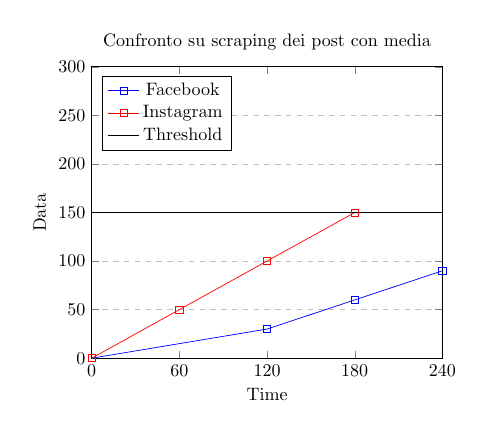
\begin{tikzpicture}[scale=0.65, transform shape]
\begin{axis}[
    title={Confronto su scraping dei post con media},
    xlabel={Time},
    ylabel={Data},
    xmin=0, xmax=240,
    ymin=0, ymax=300,
    xtick={0,60,120,180,240},
    ytick={0,50,100,150,200,250,300},
    legend pos=north west,
    ymajorgrids=true,
    grid style=dashed,
]

\addplot[
    color=blue,
    mark=square,
    ]
    coordinates {
    (0,0)(120,30)(180,60)(240,90)
    };
    \legend{Facebook}
\addplot[
    color=red,
    mark=square,
    ]
    coordinates {
    (0,0)(60,50)(120,100)(180,150)
    };
\addplot[mark=none, black,samples=2] coordinates {(0,150)(240,150)};
    \legend{Facebook, Instagram, Threshold}
\end{axis}
\end{tikzpicture}
%}
\end{column}

\begin{column}{0.5\textwidth}
\centering
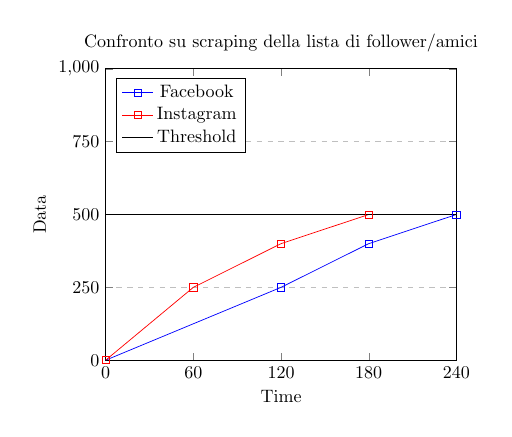
\begin{tikzpicture}[scale=0.65, transform shape]
\begin{axis}[
    title={Confronto su scraping della lista di follower/amici},
    xlabel={Time},
    ylabel={Data},
    xmin=0, xmax=240,
    ymin=0, ymax=1000,
    xtick={0,60,120,180,240},
    ytick={0,250,500,750,1000},
    legend pos=north west,
    ymajorgrids=true,
    grid style=dashed,
]

\addplot[
    color=blue,
    mark=square,
    ]
    coordinates {
    (0,0)(120,250)(180,400)(240,500)
    };
    \legend{Facebook}
\addplot[
    color=red,
    mark=square,
    ]
    coordinates {
    (0,0)(60,250)(120,400)(180,500)
    };
\addplot[mark=none, black,samples=2] coordinates {(0,500)(240,500)};
    \legend{Facebook, Instagram, Threshold}
\end{axis}
\end{tikzpicture}
\end{column}
\end{columns}
\end{frame}

\begin{frame}{Conclusioni e sviluppi futuri}
    Grazie ai connettori sviluppati si \`e garantita:
    \begin{itemize}
        \item Continuit\`a operativa dello scraping
        \item Buona elusione dei controlli
        \item Portabilit\`a del software
    \end{itemize}
    Possibili \alert{sviluppi futuri} possono basarsi su:
    \begin{itemize}
        \item Nuovi metodi di elusione (es. ``ip-rotation'') 
        \item Implementazione dei connettori in sistemi distribuiti
    \end{itemize}
\end{frame}
\begin{frame}
     \centering
     \huge{Grazie per l'attenzione}
\end{frame}